\chapter{Appendix}


\listoffigures
\listoftables

\section{Additional tables of ISBI challenge results}

%\begin{table}[H]
\begin{center}
%\caption{Results for the main submission (with postprocessing)}
\begin{minipage}{\textwidth}
\captionof{table}{Results for the main submission for the high density data set (with postprocessing)}\label{reshd1}%
\begin{tabular}{lrrrr}
Dataset&Jaccard (in \%)&Precsision (in \%)& Recall (in \%) & RMSE (in nm)\\
HD1&40.44&100&41&40.13\\
HD2&30.84&100&31&63.18\\
HD3&12.55&100&13&61.8
\end{tabular} 
\end{minipage}
\end{center}
%\end{table}


%\begin{table}[H]
\begin{center}
\begin{minipage}{\textwidth}
\captionof{table}{Results for the high precission submission for the high density data set}\label{reshd2}
\begin{tabular}{lrrrr}
Dataset&Jaccard (in \%)&Precsision (in \%)& Recall (in \%) & RMSE (in nm)\\
HD1&37.62&100&38&40.23\\
HD2&28.37&100&28&60.70\\
HD3&12.66&100&13&62.58
\end{tabular}
\end{minipage}
\end{center}
%\end{table}

\begin{center}
\begin{minipage}{\textwidth}
\captionof{table}{Results for the high score submission for the high density data set (without postprocessing)}\label{reshd3}
\begin{tabular}{lrrrr}
Dataset&Jaccard (in \%)&Precsision (in \%)& Recall (in \%) & RMSE (in nm)\\
HD1&37.96&100&38&40.22\\
HD2&29.73&94&30&63.33\\
HD3&13.00&99&13&63.95
\end{tabular}
\end{minipage}
\end{center}


\begin{center}
\begin{minipage}{\textwidth}
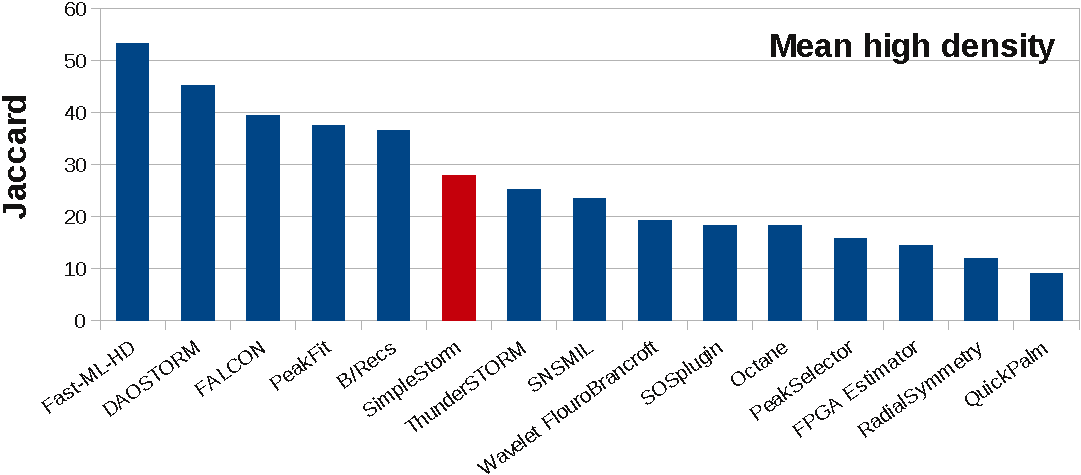
\includegraphics[width = 0.88\textwidth]{pictures/diagrammsChallenge/MeanHighDensityJaccardCropped.pdf}
	\captionof{figure}{Results for high density data sets. The Jaccard indices are averaged over all three data sets. For this score higher is better.}
	\label{meanJaccardHighDensity}
	\end{minipage}
\end{center}

\begin{center}
\begin{minipage}{\textwidth}
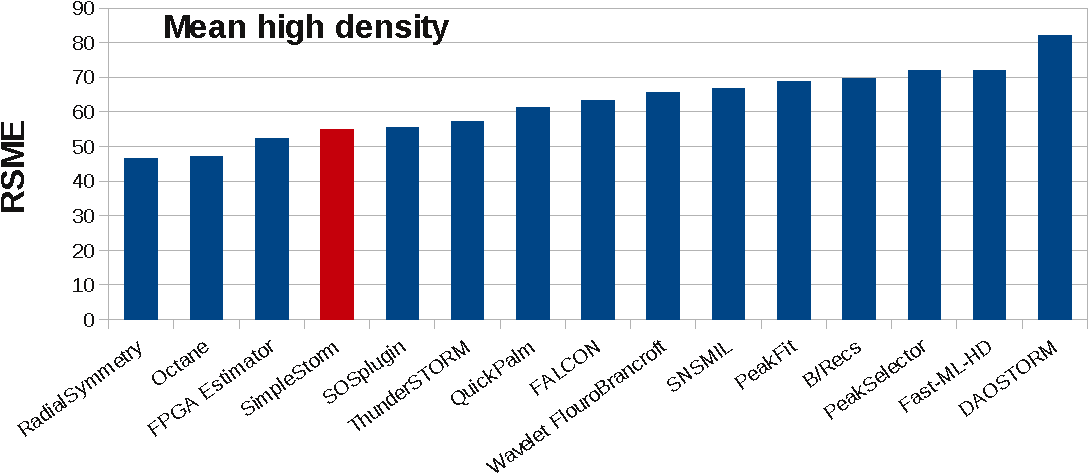
\includegraphics[width = 0.88\textwidth]{pictures/diagrammsChallenge/MeanHighDensityRSMECropped.pdf}
	\captionof{figure}{Results for high density data sets. Averaged RSME scores over all three datasets. For this score lower is better.}
	\label{meanRSMEHighDensity}
	\end{minipage}
\end{center}



\begin{center}
\begin{minipage}{\textwidth}
\captionof{table}{Results for the main submission for low density data sets(with postprocessing)}
\begin{tabular}{lrrrr}
Dataset&Jaccard (in \%)&Precsision (in \%)& Recall (in \%) & RMSE (in nm)\\
LS1&86.12&100&86&26.32\\
LS2&69.64&97&71&37.43\\
LS3&47.48&99&48&54.2
\end{tabular}\label{resls1}
\end{minipage}
\end{center}


\begin{center}
\begin{minipage}{\textwidth}
\captionof{table}{Results for the high precission submission for low density data sets}\label{resls2}
\begin{tabular}{lrrrr}
Dataset&Jaccard (in \%)&Precsision (in \%)& Recall (in \%) & RMSE (in nm)\\
LS1&83.39&100&83&27.91\\
LS2&63.21&100&63&39.57\\
LS3&40.82&100&41&49.55
\end{tabular}
\end{minipage}
\end{center}

\begin{center}
\begin{minipage}{\textwidth}
\captionof{table}{Results for the high score submission for low density data sets (without postprocessing)}\label{resls3}
\begin{tabular}{lrrrr}
Dataset&Jaccard (in \%)&Precsision (in \%)& Recall (in \%) & RMSE (in nm)\\
LS1&87.23&99&88&28.10\\
LS2&65.95&89&72&44.60\\
LS3&40.82&96&48&54.40
\end{tabular}
\end{minipage}
\end{center}



\begin{center}
\begin{minipage}{\textwidth}
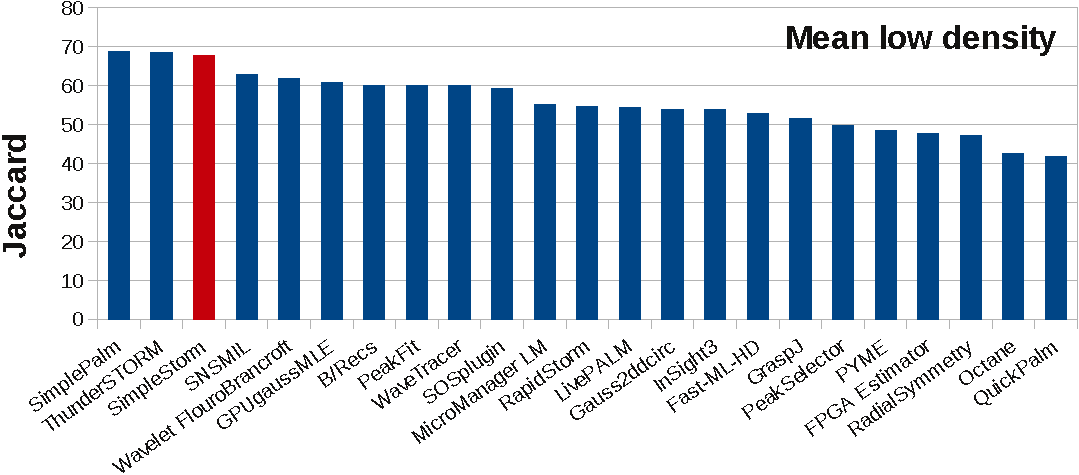
\includegraphics[width = 0.88\textwidth]{pictures/diagrammsChallenge/MeanLowDensityJaccardCropped.pdf}
	\captionof{figure}{Results for low density data sets. The Jaccard indices are averaged over all three data sets. For this score higher is better.}
	\label{meanJaccardLowDensity}
\end{minipage}
\end{center}

\begin{center}
\begin{minipage}{\textwidth}
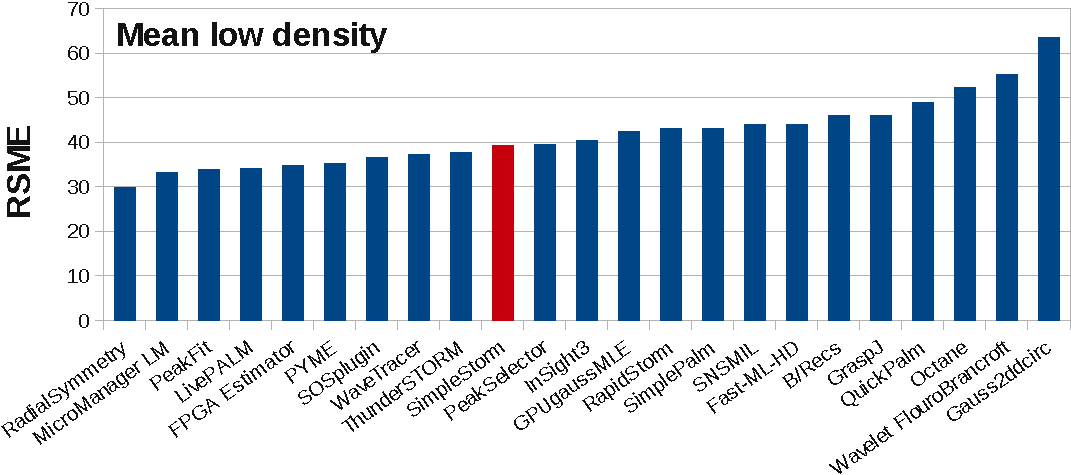
\includegraphics[width = 0.88\textwidth]{pictures/diagrammsChallenge/MeanLowDensityRSMECropped.pdf}
	\captionof{figure}{Results for low density data sets. Averaged RSME scores over all three datasets. For this score lower is better.}
	\label{meanRSMELowDensity}
\end{minipage}
\end{center}

\begin{center}
\begin{minipage}{\textwidth}
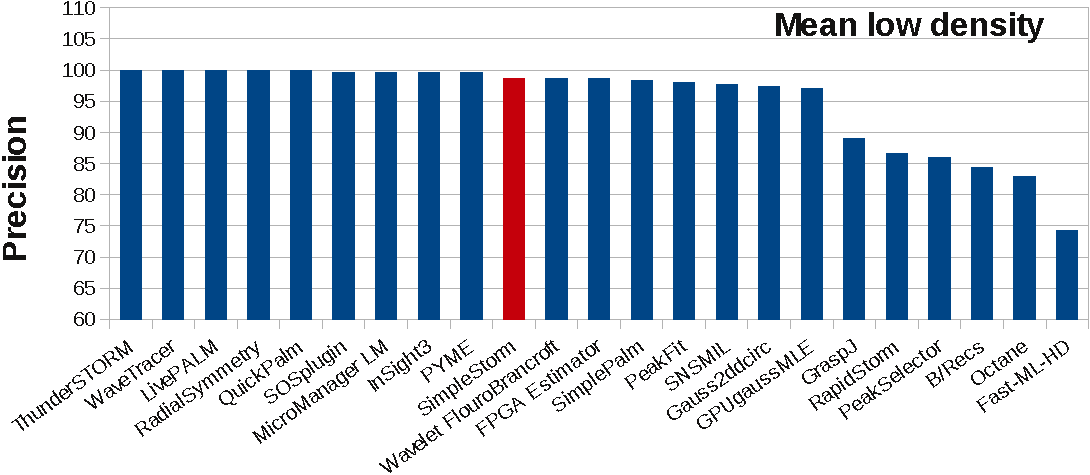
\includegraphics[width = 0.88\textwidth]{pictures/diagrammsChallenge/MeanLowDensityPrecisionCropped.pdf}
	\captionof{figure}{Results for low density data sets. Averaged Precision over all three datasets. For this score higher is better. The y axis is broken to show the differences better.}
	\label{meanPrecisionLowDensity}
\end{minipage}
\end{center}

\begin{center}
\begin{minipage}{\textwidth}
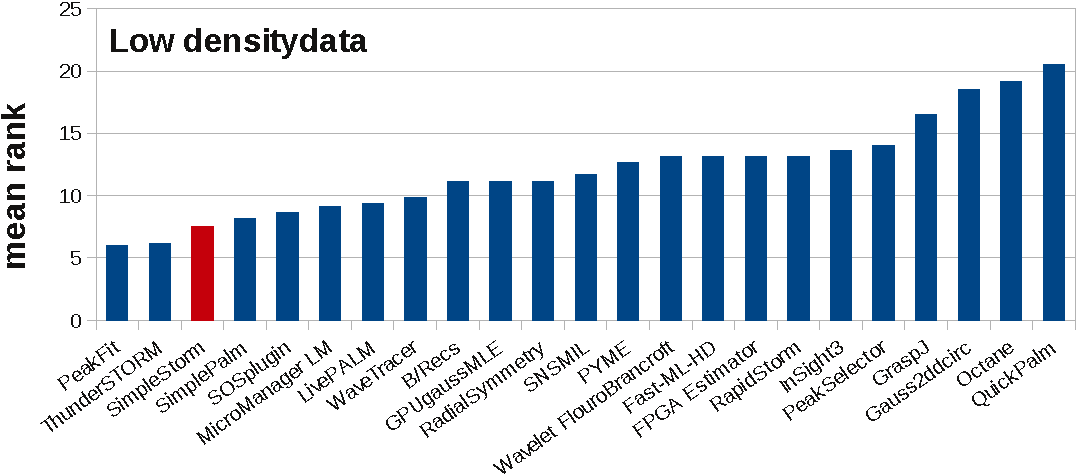
\includegraphics[width = 0.88\textwidth]{pictures/diagrammsChallenge/MeanRankLowDensityCropped.pdf}
	\captionof{figure}{Averaged rank over Jaccard index and RSME score for all low density data sets. Lower ranks are better.}
	\label{meanRankLow}
\end{minipage}
\end{center}

\begin{center}
\begin{minipage}{\textwidth}
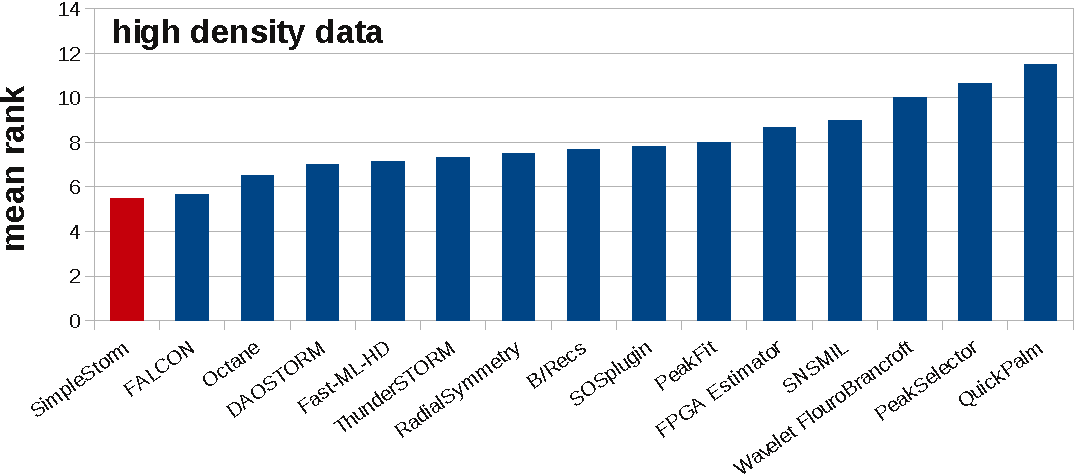
\includegraphics[width = 0.88\textwidth]{pictures/diagrammsChallenge/MeanRankHighDensityCropped.pdf}
	\captionof{figure}{Averaged rank over Jaccard index and RSME score for all high density data sets. Lower ranks are better}
	\label{meanRankHigh}
	\end{minipage}
\end{center}